\documentclass{article}
\usepackage{graphicx} % Required for inserting images
\usepackage{titlesec}
\usepackage{tabularx}
\usepackage{makecell} 
\usepackage{array} 
\usepackage{enumitem}
\usepackage{changepage}  
\usepackage{geometry}
\usepackage{float}
\usepackage[none]{hyphenat}
\setcounter{secnumdepth}{4}

\titleformat{\paragraph}
{\normalfont\normalsize\bfseries}{\theparagraph}{1em}{}
\titlespacing*{\paragraph}
{0pt}{3.25ex plus 1ex minus .2ex}{1.5ex plus .2ex}

\title{\textbf{Design Document}}
\author{Armando Fiorini, Samuele Motta, Vajihe Gholami}
\date{}

\begin{document}

\maketitle
\section*{INFO}
\textbf{Deliverable}: DD\\
\textbf{Title}: Design Document\\
\textbf{Authors:} Armando Fiorini, Samuele Motta, Vajihe Gholami\\
\textbf{Version:} 0.0.0\\
\textbf{Date}: 17/12/2023\\
\textbf{Download page}: https://github.com/ArmaFio/FioriniMottaGholami\\
\newpage
\tableofcontents
\newpage

\section{Introduction}
\subsection{Purpose}
The main purpose of the present document is to support the development team in realizing the system. It provides an overall description of the adopted system architecture and a breakdown of the various components to a significant extent, also describing their interactions with each other. On top of that, the Design Document (DD) describes the implementation, integration, and testing plans which are defined keeping into account priority, required effort, and impact of the single components on the stakeholders.

\subsection{Scope}
CodeKataBattle (CKB) helps students improve their software skills through teamwork on coding challenges. It's all about learning together in a fun, competitive way. Educators create tournaments with coding exercises, and students form teams to solve them. The platform handles everything: deadlines, tests, and checking code quality.

Educators can also give personal feedback and scores. CKB is where educators set challenges, students solve them as teams, and everyone can see how they're doing. It handles tournaments, battles, team setups, code submissions via GitHub, live scoring, and awarding badges for achievements.

The system focuses on teamwork, good coding methods using tests, and a mix of competition and support. Automated tools ensure fair assessments while letting educators give helpful feedback. Badges and student profiles make it fun, encouraging everyone to participate and shine. Overall, CKB is a platform mixing learning, teamwork, competition, and skill-building in software development.

\subsection{Definitions, Acronyms, Abbreviations}
\subsubsection{Definitions}
Educator: A user who signs up to use the system to improve his students' programming skills can create Tournaments and badges. \\
Student: user who signs up to improve their skills, and participate in tournaments are created by the educators.\\
Tournament: coding challenge, consisting of a certain number of battles. Team: group of students, formed to join a tournament and work together to win the battles. \\
Battle: every single challenge the tournament is composed of. \\
(Gamification) Badge: achievement that is created by an educator, and can be obtained from Students satisfying the established requirements.\\

\subsubsection{Acronyms}
\begin{itemize}
    \item \textbf{CKB}: CodeKataBattle
    \item \textbf{RASD}: Requirement Analysis and Specification Document
    \item \textbf{UI}: User Interface
    \item \textbf{UML}: Unified Modelling Language
    \item \textbf{OS}: Operative System
\end{itemize}

\subsection{Revision History}
\begin{itemize}
    \item \textbf{$[Gn]$}: the n-th goal of the system.
    \item \textbf{$[Wn]$}: the n-th world phenomena.
    \item \textbf{$[SWn]$}: the n-th shared phenomena controlled by the world.
    \item \textbf{$[SMn]$}: the n-th shared phenomena controlled by the machine.
    \item \textbf{$[Dn]$}: the n-th domain assumption.
    \item \textbf{$[FRn]$}: the n-th functional requirement.
\end{itemize}


\subsection{Reference Documents}
This document is based on:
\begin{itemize}
    \item The specification of the RASD and DD assignment of the Software Engineering II course, held by Professor Matteo Rossi, Elisabetta Di Nitto, and Matteo Camilli at the Politecnico di Milano, A.Y 2023/2024; 
    \item Slides of Software Engineering 2 course on WeBeep;
\end{itemize}


\subsection{Document Structure}
Mainly the current document is divided into 4 chapters, which are:
\begin{itemize}
    \item \textbf{Introduction:} The first chapter includes the introduction which explains the purpose of the document, then, a brief recall of the concepts introduced in the RASD is given. Finally, important information for the reader is given, i.e. definitions, acronyms, synonyms, and the set of documents referenced. 
    \item \textbf{Architectural Design:} It includes a detailed description of the architecture of the system, including the high-level view of the elements, the software components of …, a description through run-time diagrams of various functionalities of the system, and, finally, an in-depth explanation of the architectural pattern used.
    \item \textbf{User Interface Design:} Provide mockups of the application user interfaces, with the links between them to help in understanding the flow between them. 
    \item \textbf{Requirements Traceability:} It describes the connections between the requirements defined in the RASD and the components described in the first chapter. This is used as proof that the design decisions have been taken concerning the requirements, and therefore that the designed system can fulfill the goals. 
    \item \textbf{Implementation, Integration, and Test Plan:} It describes the process of implementation, integration, and testing to which developers have to stick to produce the correct system correctly. 
    \item \textbf{Effort Spent:} Contains information about the time spent to create this document. 
    \item \textbf{References:} It contains the references to any documents and the Software used in this document. 
\end{itemize}
\section{Architectural Design}

\subsection{Overview}
This section gives an overview of the architectural elements that compose the system, their interaction, and a description of the replication mechanism chosen for the system to make it distributed.
\subsection{High-Level view}

The CodeKataBattle project follows a 3-tier architecture, segregating its functionalities into distinct layers. (Figure \ref{fig:3-tier}) The Presentation Layer handles the user interface, authentication, notifications, and badge visualization. The Application Layer contains the core logic, managing battles, tournaments, GitHub integration, score calculation, and badge generation. The Data Layer ensures data integrity and storage, interacting with the database and employing ORM for data operations. Communication between these tiers occurs through APIs or service calls. This modular structure streamlines development, fostering scalability and maintainability. The front end allows user interaction while the back end manages logic, data, and integrations, providing educators and students with a seamless platform to engage in code kata battles and tournaments, track progress, and visualize achievements through earned badges.

\begin{figure}[H]
    \centering
    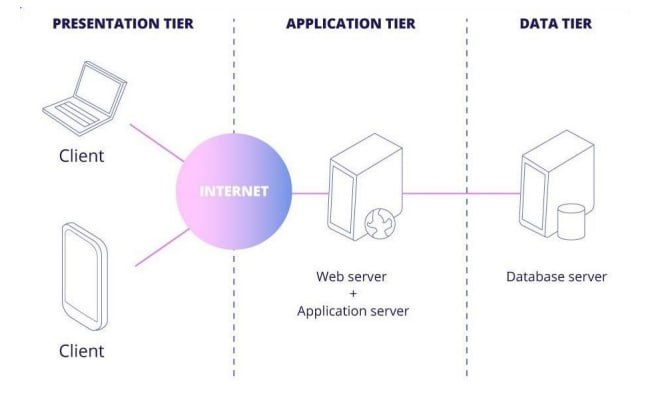
\includegraphics[width=\linewidth]{High level view.jpg}
    \caption{3-tier architecture}
    \label{fig:3-tier}
\end{figure}

Regardless of whether the user is an educator or a student, they can access the application through either the web or mobile app, with communication between the client and server relying on various components tailored to the consumer device's type.

\begin{figure}[H]
    \centering
    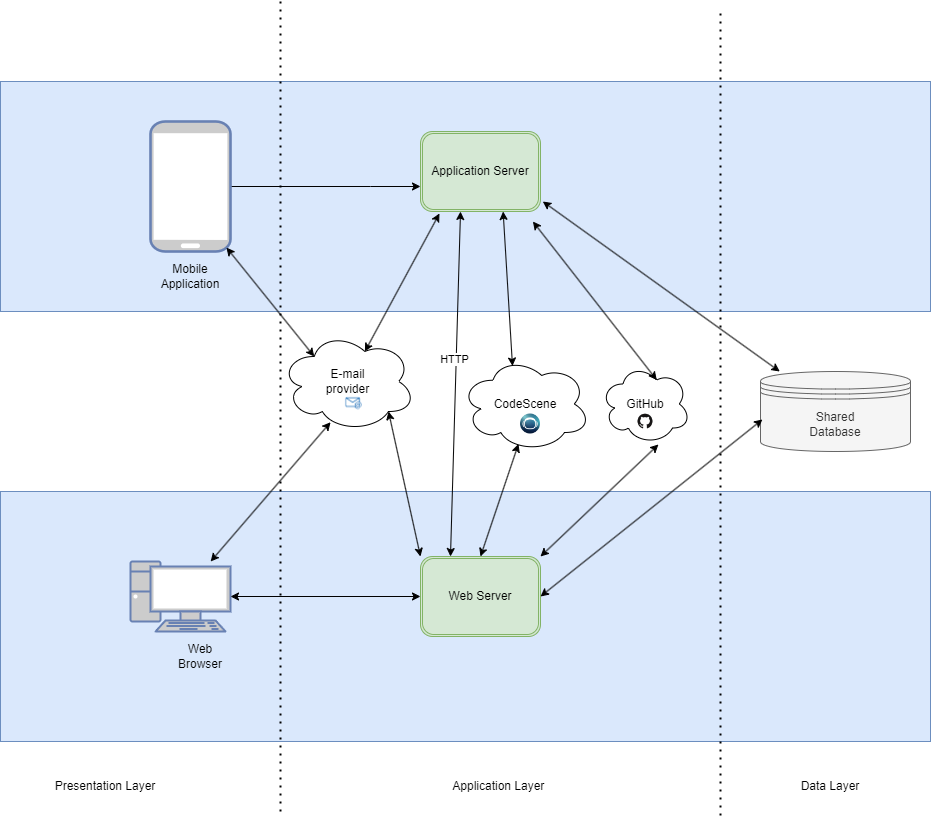
\includegraphics[width=\linewidth]{HighLevelSystemArchitecture.png}
    \caption{High Level System Architecture}
\end{figure}
\newpage

\subsection{Component view}
This section provides a description of the system's component diagram, outlining all internal and external elements.

\begin{figure}[H]
    \centering
    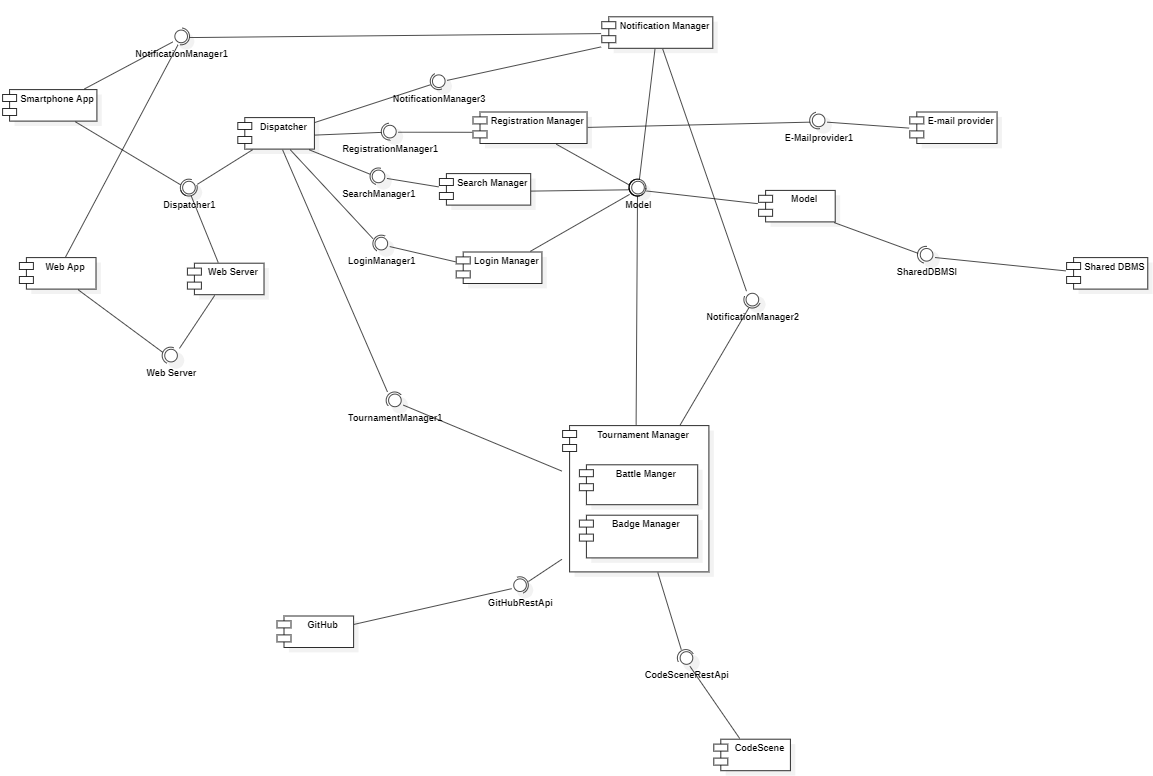
\includegraphics[width=\linewidth]{Component diagram.png}
    \caption{Component Diagram}
\end{figure}
\begin{itemize}
    \item \textbf{Smartphone App}: it's the application that needs to be installed on a mobile device to 
    get access to the system.\\
    The Smartphone App can communicate directly with the application server: every request made by it is sent to the dispatcher, which will provide to return the corresponding answer.
    \item \textbf{Web App}: it's the web version of the CKB Application, which can be accessed from an internet browser: it's connected to the application server through the web server which handles the requests before forwarding them to the dispatcher.
    \item \textbf{Web Server}: it's the component which connects the Web Application with the Application Server: the Web Server acts as a link between the Web Application and the Dispatcher, to which it forwards all the requests made by the first one, receiving the corresponding answers. 
    \item \textbf{Dispatcher}: the Dispatcher receives all the requests from the Smartphone App and the web server and manages them contacting the corresponding component: when the request has been correctly processed it returns the answer to the caller.
    \item \textbf{Login Manager}: this component handles all the login requests made by users of the system: it checks the credentials and, if they are correct, sends the Dispatcher the corresponding account data to fill the user's dashboard.
    \item \textbf{Registration Manager}: this component handles the registration procedures for new users of the system: it checks the availability of the credentials they want to use and if they are available it manages the creation of the new account and sends to the Dispatcher the confirmation of the completion of the registration.
    This component interacts with the \textbf{E-mail provider} to handle the procedure of user's e-mail confirmation, when a new account is being created.
    \item \textbf{Tournament Manager}: this component handles the management of all concerning the tournaments creation, conduction and closure.\\
    The tournament manager has got two subcomponents used to handle some specific aspects of the tournament: in particular the creation and management of the single battles are handled by the \textbf{Battle Manager}, which uses also the connections with \textbf{GitHub} and \textbf{CodeScene} to create the repository for the battle and evaluate the students' solutions for the battle, the creation and assignments of the badges are instead handled by the \textbf{Badge Manager}.
    \item \textbf{Search Manager}: the search manager manages all the request of account searching and visualizing: it takes from the database the requested accounts or list and returns them to the dispatcher to be shown to the user.
    \item \textbf{Notification Manager}: the notification manager manages the creation and the storing and visualization of notifications: it is directly linked to the Tournament Manager which uses his interface when a notification about a tournament itself has to be sent to one or more users.\\
    This component is also connected to the model and dispatcher to manage the notifications visualization requests: when an user accesses the notifications section in the mobile/web application, a request for the list of pending notifications is sent to the system and forwarded by the dispatcher to the notification manager which takes the data from the DBMS
    \item \textbf{Model}: the Model is the component of the system which contains all the representations of entities involved in the system: when some data has to be taken from the DBMS the task is assigned to the model which stores them in the appropriate data structure.
    The model also offers the methods which are necessary to modify, manipulate and interact with the entities of the system.
    It's the only component which can directly interact with the DBMS.
    \item \textbf{Shared DBMS}: the DBMS is used to store all the data regarding all the tournaments, battles, users of the system.
    This component solves queries and returns the data to the model to be stored in the system through the data structures provided by the model.
\end{itemize}
\subsection{Deployment view}
This chapter provides insights into the deployment view of CKB, detailed in \textbf{Figure 3}. Within this view, we delve into the execution environment of the system, elucidating the physical distribution of the hardware components responsible for executing the software that forms the application.
\begin{figure}[H]
    \centering
    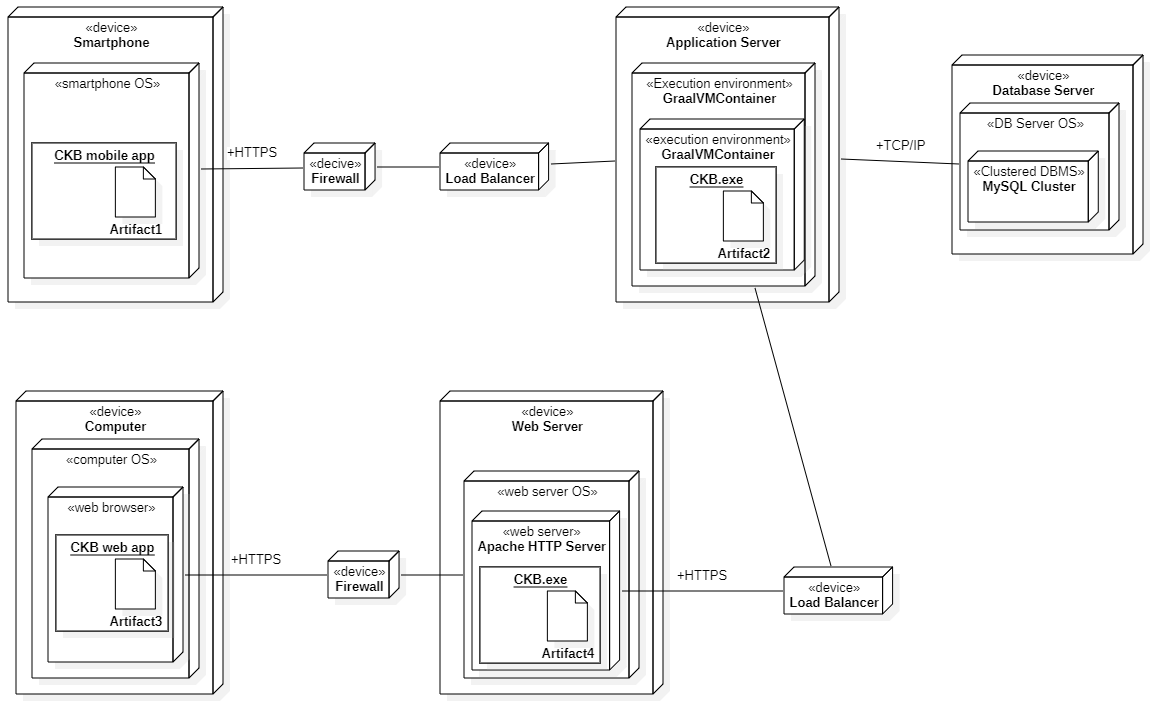
\includegraphics[width=\linewidth]{deployment diagram.png}
    \caption{System Deployment View}
\end{figure}
\noindent
Additional intricacies about the elements depicted in the graph are elaborated in the following sections.
\begin{itemize}
    \item \textbf{Smartphone} \\
    The smartphone, acting as a client, has the capability to install the CKB app. Communication between the software and the system occurs through HTTPS requests, which are directly transmitted to the Application Server without passing through the Web Server.
    \item \textbf{Computer} \\
    The computer is a standard device with internet access through a web browser. Users will utilize the web browser to explore the internet and locate the CKB webpage. Via an HTTPS request, the web server accesses the Application Server, forwarding the request to provide the required service.
    \item \textbf{Firewall} \\
    The firewall, positioned before the two load balancers, monitors incoming packets to the system. If a packet is deemed potentially dangerous, it is not forwarded. This setup ensures that only safe packets enter the network, creating a Demilitarized Zone (DMZ) that encompasses all elements, except for smartphones and computers.
    \item \textbf{Load Balancer} \\
    A load balancer efficiently distributes incoming network traffic across multiple servers, optimizing performance, preventing overload, and enhancing system reliability by redirecting requests to less burdened servers. It plays a key role in scaling applications and ensuring high availability in modern computing environments.
    \item \textbf{Web Server} \\
    The web server handles all requests from users accessing the CKB web application via a web browser. It forwards these requests to the application server for processing. Once the application server returns the results of the required computations, the web server generates the corresponding web page and forwards it to the user. Alternatively, if the user's request is for a static web page, the web server returns it directly without involving the application server.
    \item \textbf{Application Server} \\
    The application server, the central component of the application tier, plays a crucial role. It receives all requests forwarded by computers via the web server and from smartphones, processes them, and retrieves the necessary information, potentially accessing the database. Importantly, the application server is the sole component with the capability to access the Database Server through a TCP/IP request.
    \item \textbf{Database Server} \\
    The database server consists of a cluster implemented through MySQL Cluster, designed to ensure data reliability, scalability, and the distribution and replication of data across multiple nodes for optimal availability and fault tolerance.
\end{itemize}

\subsection{Runtime view}
It's crucial to clarify a key point about the following sequence diagrams: the system can be accessed through both a mobile app and a web app. For simplicity, we've unified the representation of the web app and mobile app under the \textbf{App} component, omitting the web server. It's implicit that when using the web app, all requests pass through the web server before reaching other components.

\begin{figure}[H]
    \centering
    \textbf{[UC11] Manual Evaluation} \\
    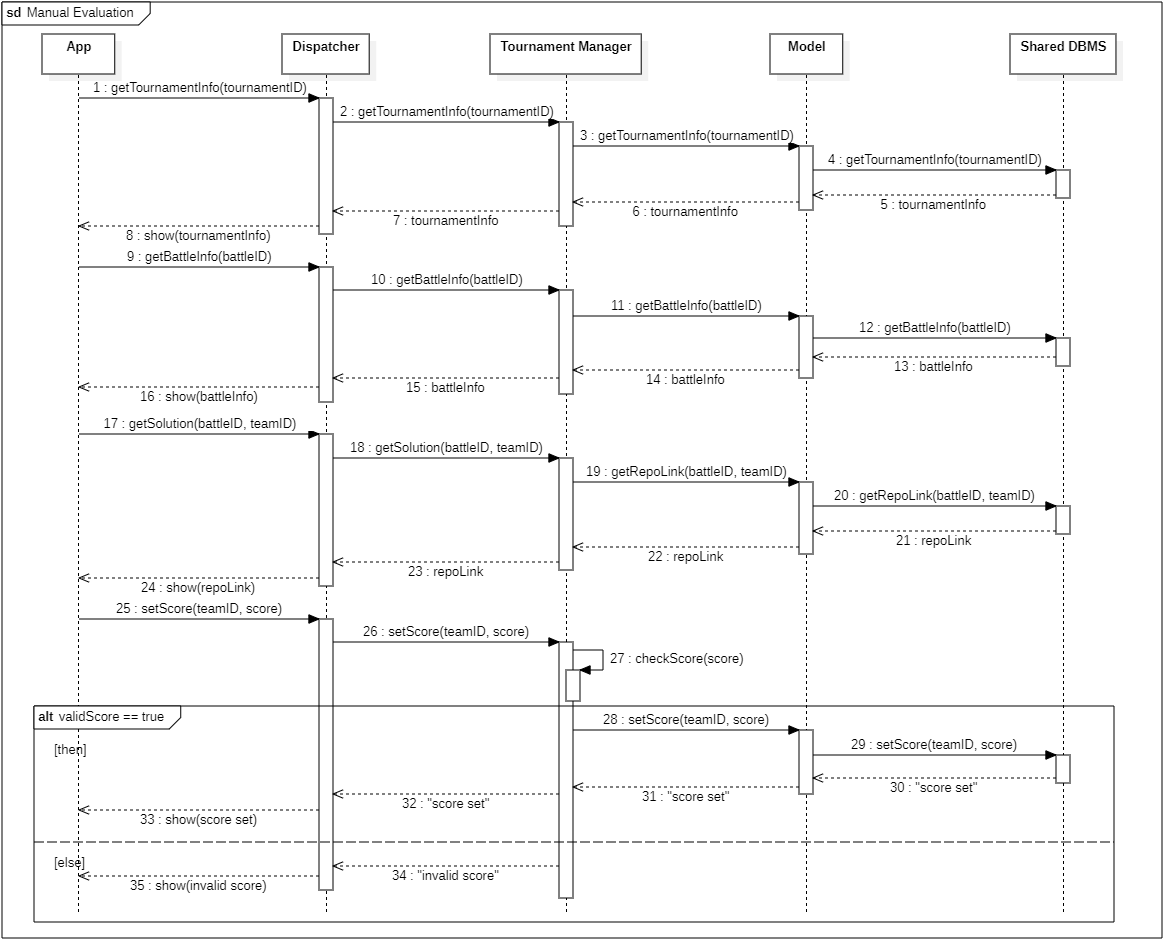
\includegraphics[width=\linewidth]{UC11.png}
\end{figure}
\noindent
This sequence diagram depicts the manual evaluation process conducted by an educator. The app initiates the procedure by sending the dispatcher a request to obtain information about a specific tournament. This request is then forwarded to the Tournament Manager, and subsequently to the Model and the Shared DBMS. \\
Once the tournament information has been retrieved, a new request is sent to the Shared DBMS to retrieve information about a specific battle within the tournament. Following this, another request is made to obtain the solution of a specific team within the battle. \\
The educator assesses the solution and assigns a score, which the Tournament Manager then verifies. If the score is deemed valid, the Tournament Manager proceeds to set the score for the solution in the Shared DBMS. Otherwise, it returns an error message to the app. \\


\begin{figure}[H]
    \centering
    \textbf{[UC12] Fork Creation} \\
    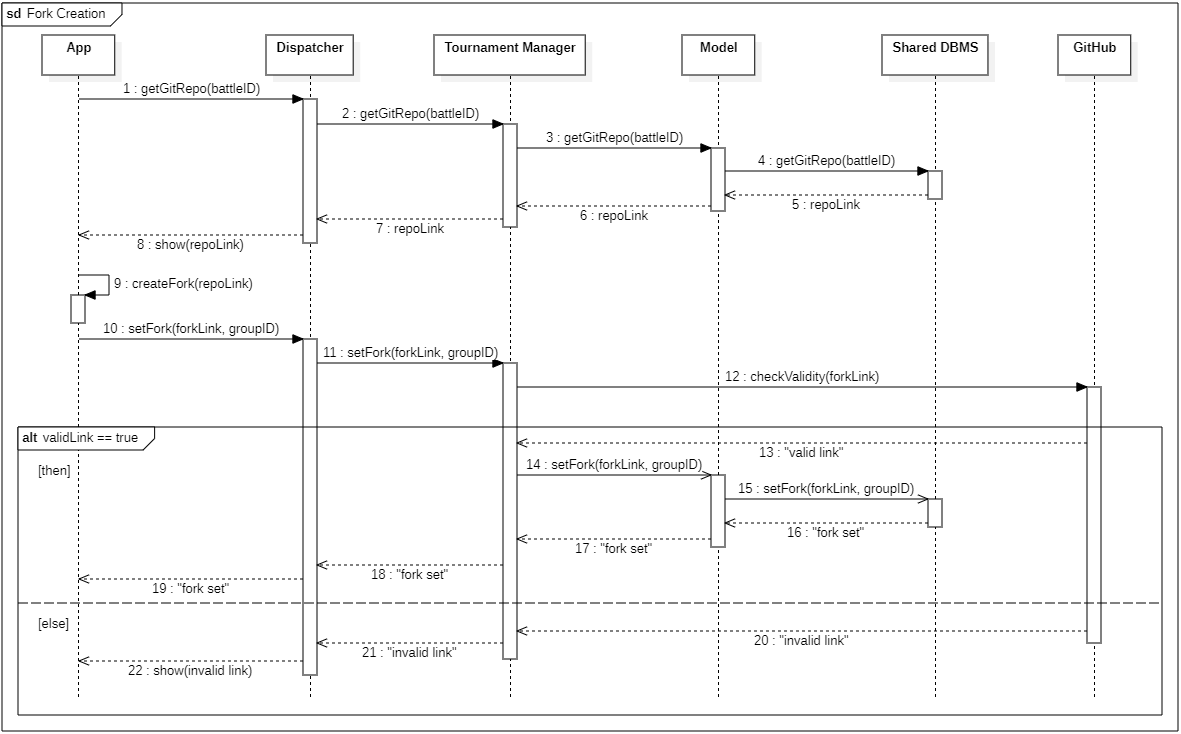
\includegraphics[width=\linewidth]{UC12.png}
\end{figure}
\noindent
This sequence diagram illustrates the fork creation process carried out by a student. The procedure commences with the app sending a request to obtain the repository link containing the problem for a specific battle. The Tournament Manager then retrieves this link from the Shared DBMS. \\
Subsequently, the student creates a new fork by accessing the GitHub repository through the provided link. The student then submits the link of the new fork to the system for processing. The Tournament Manager, in turn, interacts with the GitHub API to validate the link provided by the student. If the link is valid, the Tournament Manager saves it in the Shared DBMS and sends a confirmation message to the user. However, if the link is invalid, the system sends an error message to the user.

\begin{figure}[H]
    \centering
    \textbf{[UC13] Close Tournament} \\
    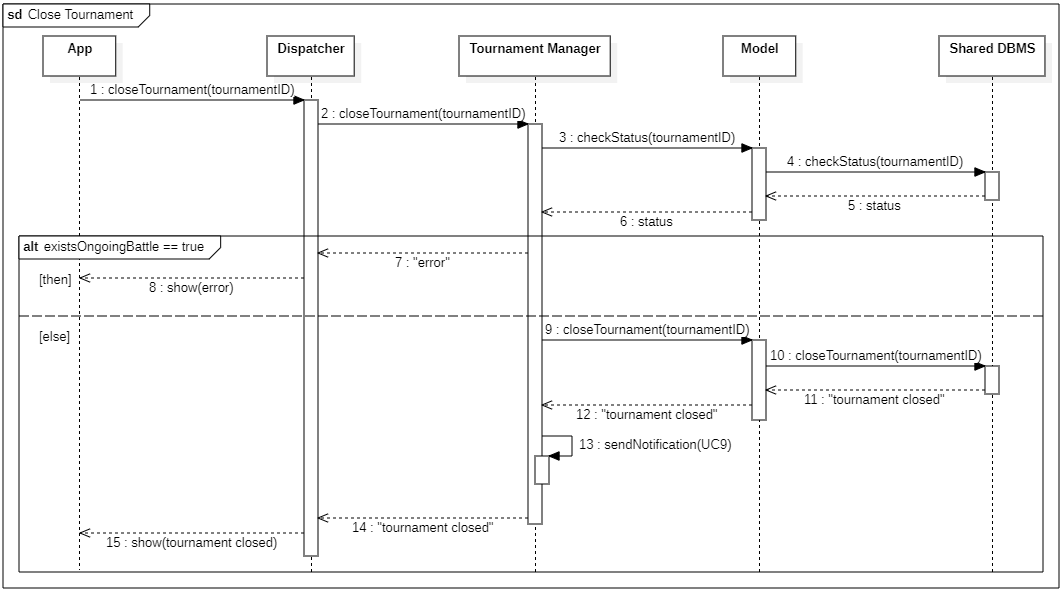
\includegraphics[width=\linewidth]{UC13.png}
\end{figure}
\noindent
This sequence diagram represents the procedure for closing a tournament, executed by the educator who created it. Initially, the app sends a request to close the tournament to the Tournament Manager, which then verifies the tournament's state through the Shared DBMS. If there are no ongoing battles within the tournament, the Tournament Manager updates the tournament state to 'closed' in the Shared DBMS and notifies all students who joined that tournament via the Notification Manager. However, if there are ongoing battles, an error message is sent to the app.

\begin{figure}[H]
    \centering
    \textbf{[UC14] Visit Profile} \\
    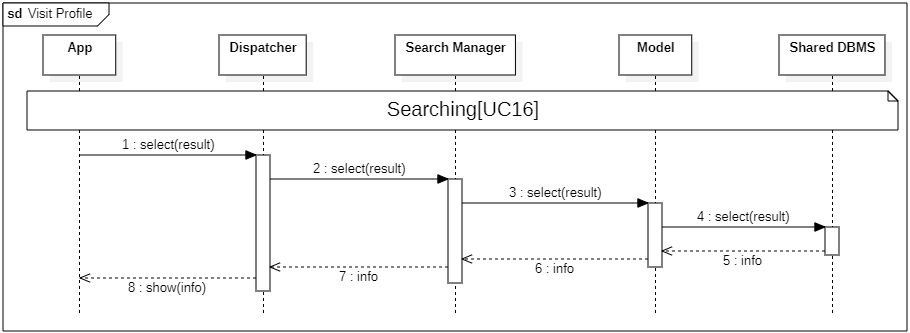
\includegraphics[width=\linewidth]{UC14.png}
\end{figure}
\noindent
This sequence diagram illustrates the process of visiting a user profile. It begins with the app initiating a request to retrieve information about a specific keyword, as described in \textbf{[UC16]}. Following the retrieval of suggested results, the app sends the selected topic to the Search Manager for information retrieval. The Search Manager then collects the information by querying the Shared DBMS. Finally, all the gathered information is sent back to the Search Manager and subsequently to the app.

\begin{figure}[H]
    \centering
    \textbf{[UC15] Joining Invitation} \\
    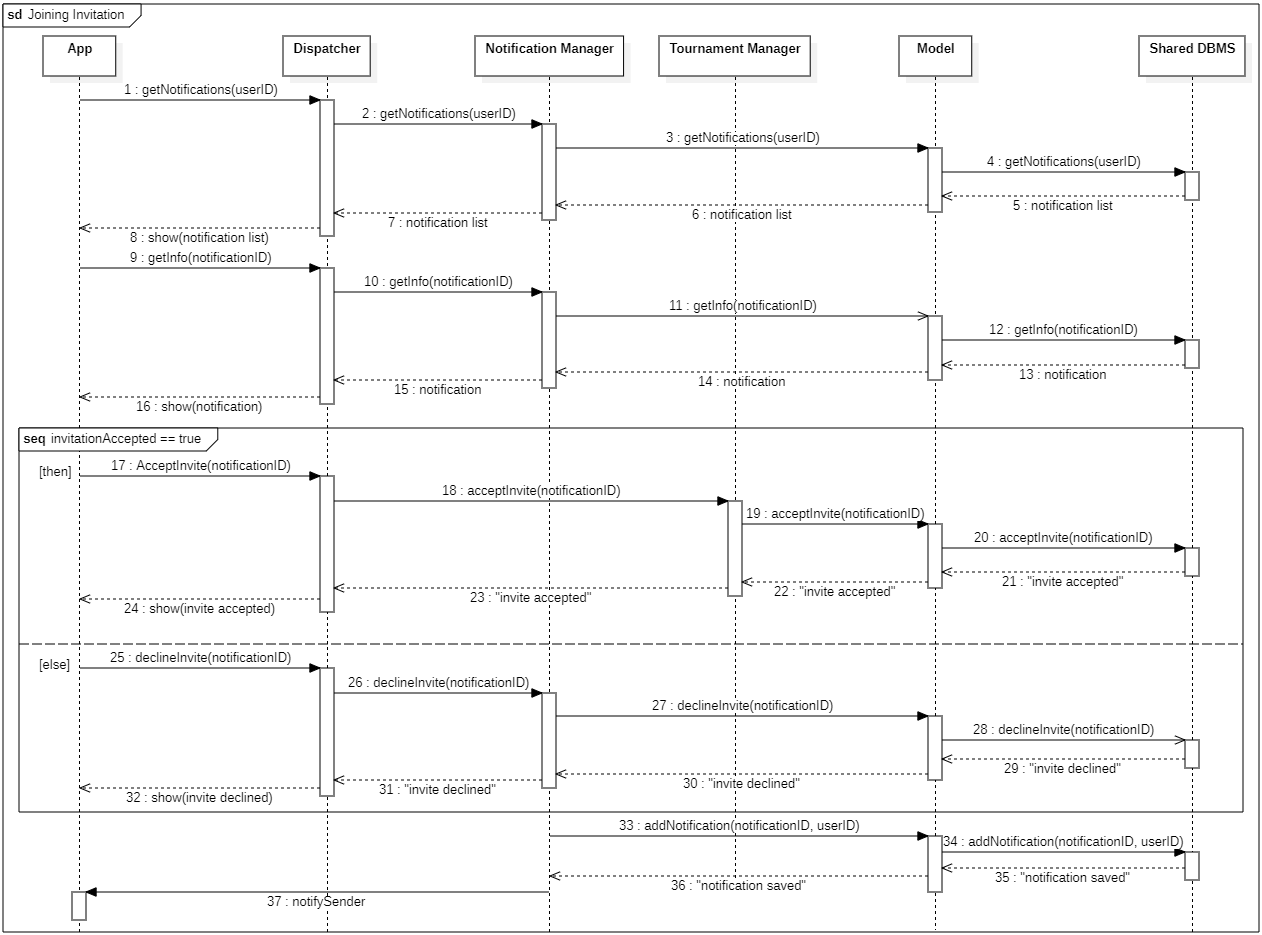
\includegraphics[width=\linewidth]{UC15.png}
\end{figure}
\noindent
This sequence diagram outlines the process of a user joining an invitation. Initially, the app sends a request to the Notification Manager to retrieve all active notifications from the Shared DBMS. Subsequently, the app requests information about a specific notification from the Notification Manager, which obtains the information by accessing the Shared DBMS. \\
If the user chooses to accept the invitation, the app sends a request to the Tournament Manager, which adds the user to the invited group. In the case of declining the invitation, the app sends a request to the Notification Manager, which handles the decline process. After the invitation is either accepted or declined, the Notification Manager creates a new notification, saves it in the Shared DBMS, and then sends the new notification to all designated users.

\begin{figure}[H]
    \centering
    \textbf{[UC16] Searching} \\
    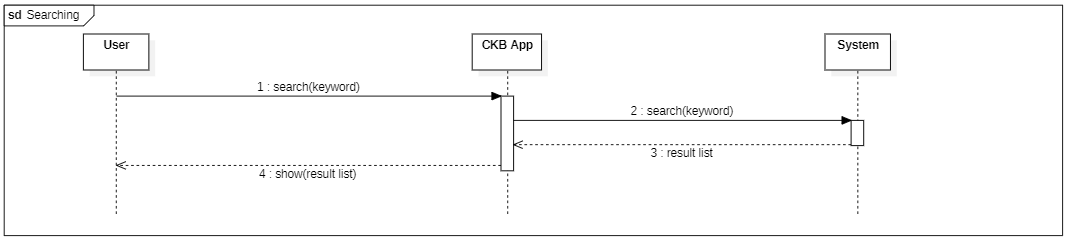
\includegraphics[width=\linewidth]{UC16.png}
\end{figure}
\noindent
This sequence diagram illustrates the user's search procedure involving the insertion of a specific keyword. The app sends a request to the Search Manager, which queries the Shared DBMS to retrieve a list of results for the specified keyword. The Search Manager then sends this list to the app.

\subsection{Component interfaces}

\subsection{Selected architectural styles and patterns}
\subsubsection{3-tier Architecture}
CKB will be built upon a 3-tier architecture, providing numerous benefits through the modularization of the system into three independent layers or tiers:
\begin{itemize}
    \item \textbf{Presentation Tier:} This top-level tier encompasses the customer interface, focusing on rearranging data received from the application tier to present it in a more intuitive and comprehensible manner to customers.
    \item \textbf{Application Tier:} This tier houses the logic of the application, governing decision-making and calculations. It plays a crucial role in passing and processing data between the surrounding layers.
    \item \textbf{Data Tier:} This tier incorporates the Database system and offers an API to the application tier for accessing and managing data stored in the database.
\end{itemize}
Adopting this architecture ensures heightened flexibility by allowing the development and updating of specific parts of the system independently. Additionally, the middle tier between the client and data server enhances data security, as information is accessed through the application layer rather than directly by the client.

\begin{itemize}
    \item MVC
    \item Observer
    \item Mediator
\end{itemize}

\subsection{Other design decisions}


\section{User Interface Design}


\begin{figure}[H]
    \centering
    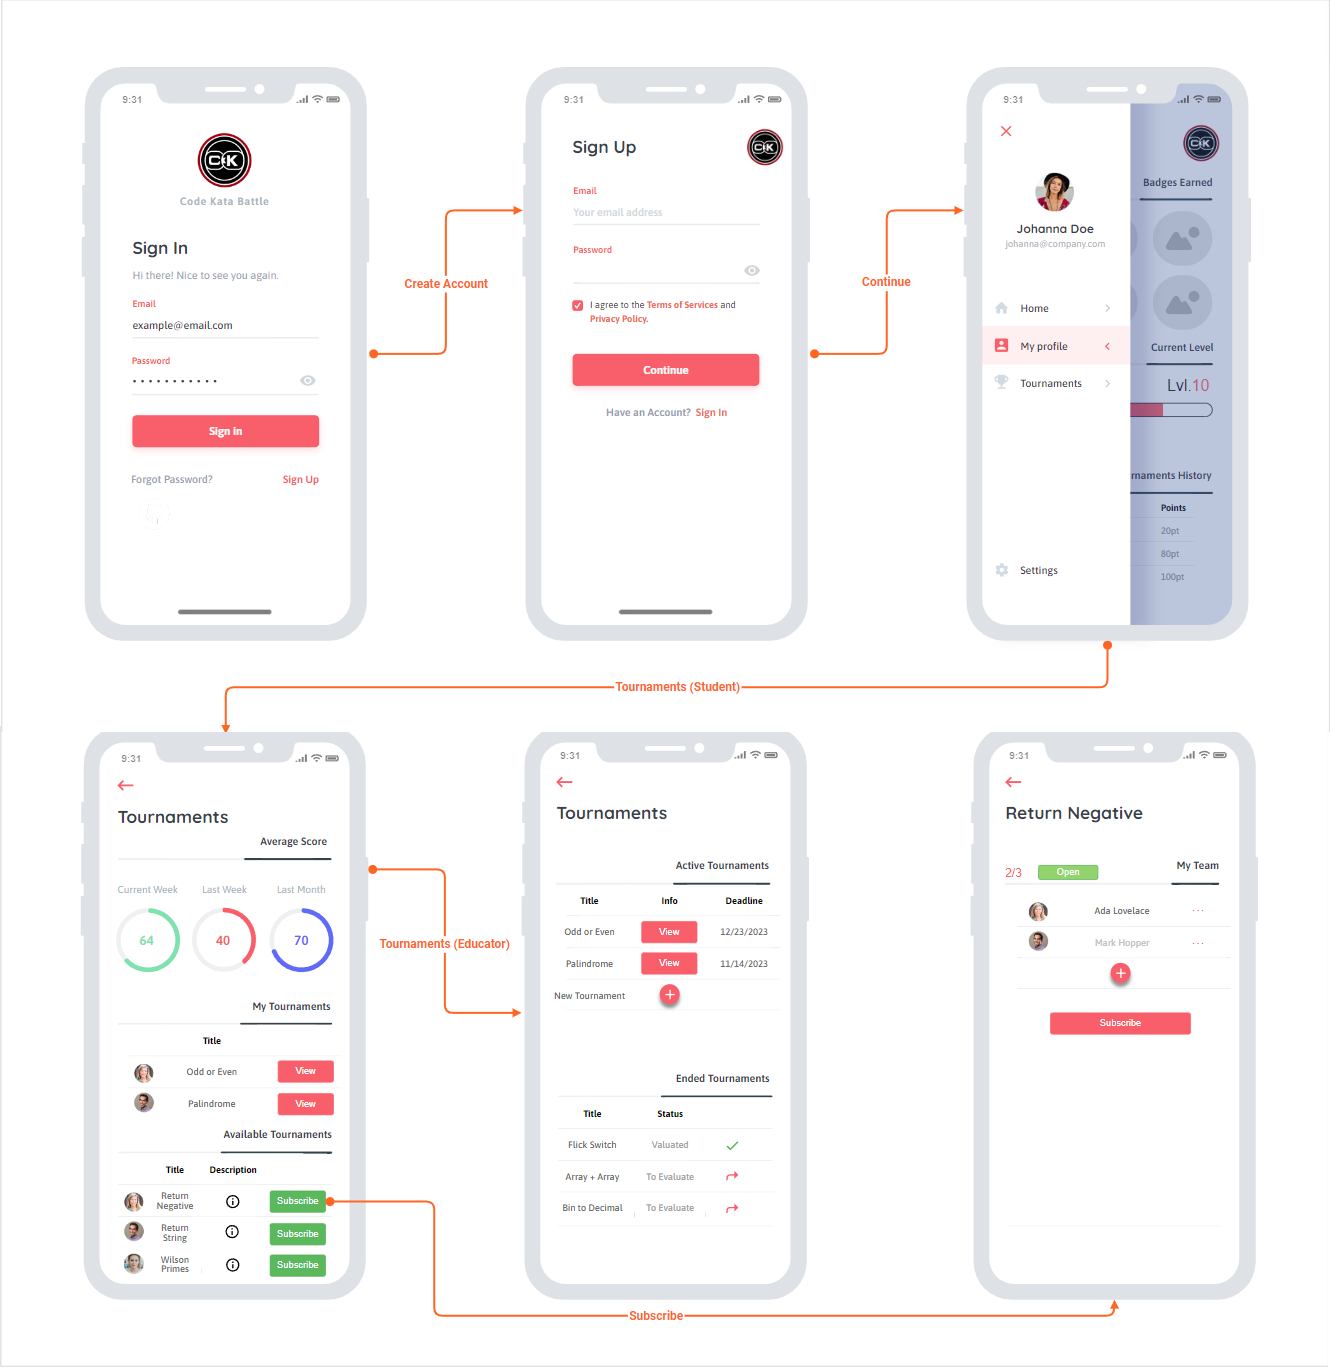
\includegraphics[width=\linewidth]{Mobile UI.png}
    \caption{General UI}
\end{figure}

\begin{figure}[H]
    \centering
    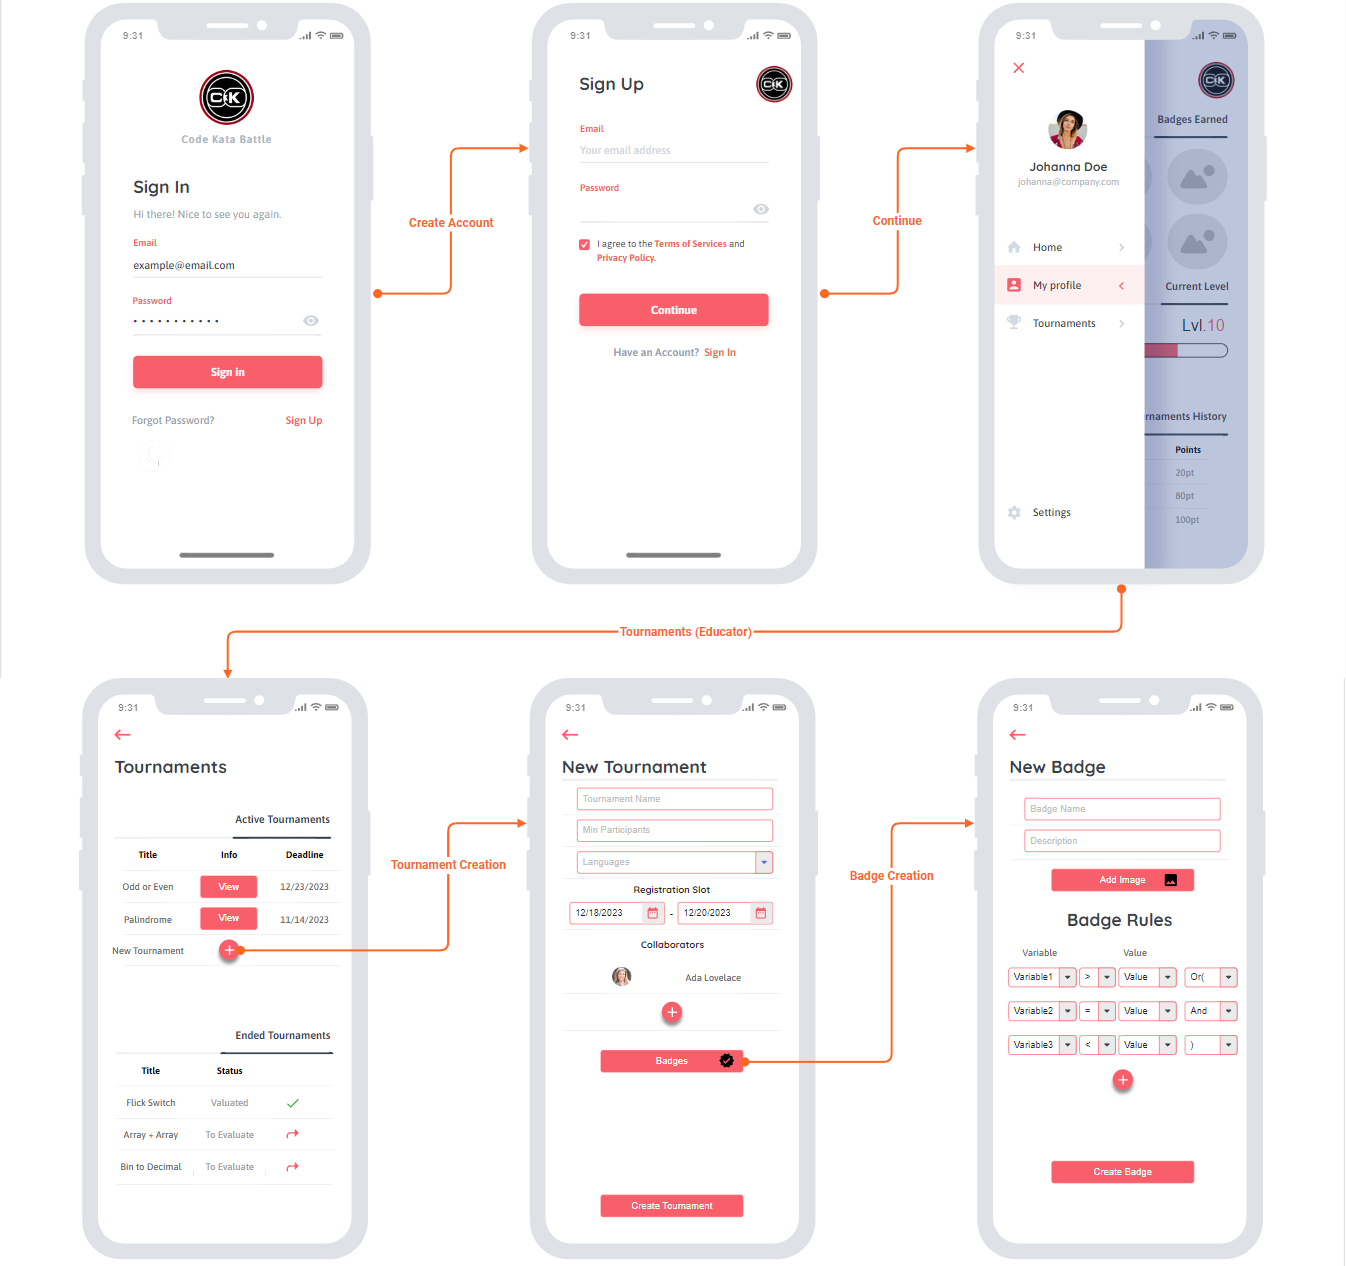
\includegraphics[width=\linewidth]{Mobile UI ED.png}
    \caption{Tournament and Badge creation}
\end{figure}

\begin{figure}[H]
    \centering
    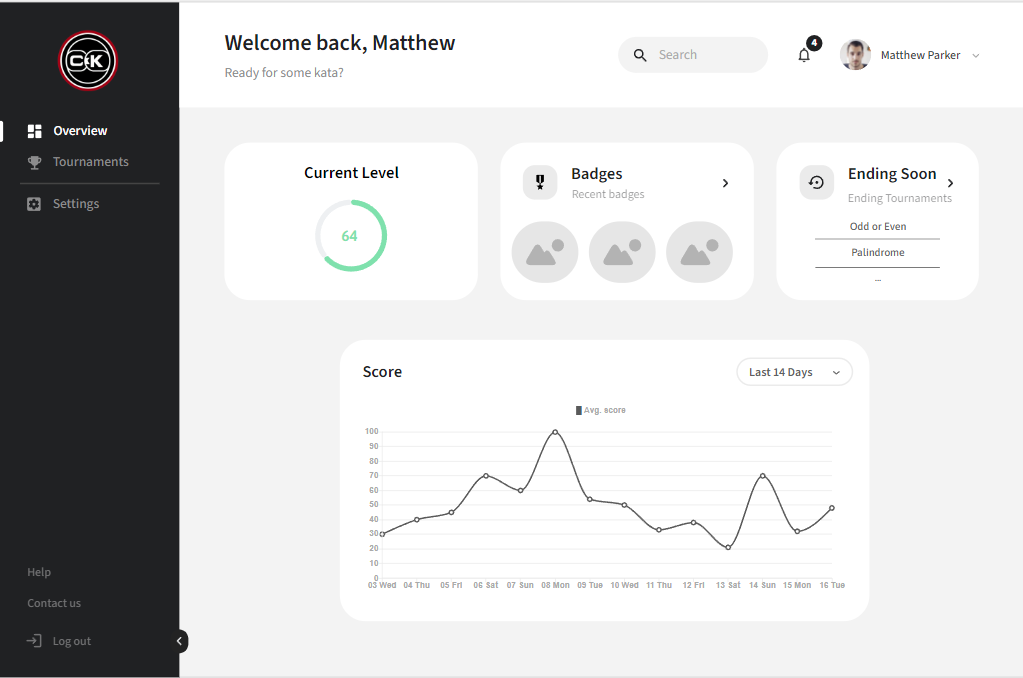
\includegraphics[width=\linewidth]{Web UI.png}
    \caption{Web UI Overview}
\end{figure}

\begin{figure}[H]
    \centering
    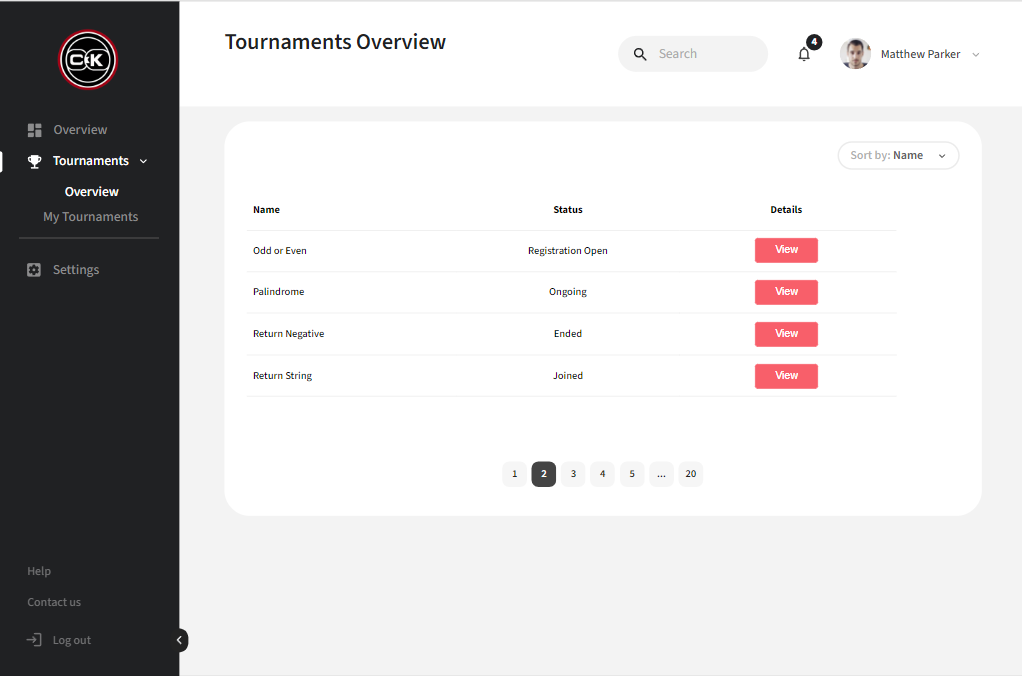
\includegraphics[width=\linewidth]{Web UI 2.png}
    \caption{Web UI Tournament Overview}
\end{figure}

\begin{figure}[H]
    \centering
    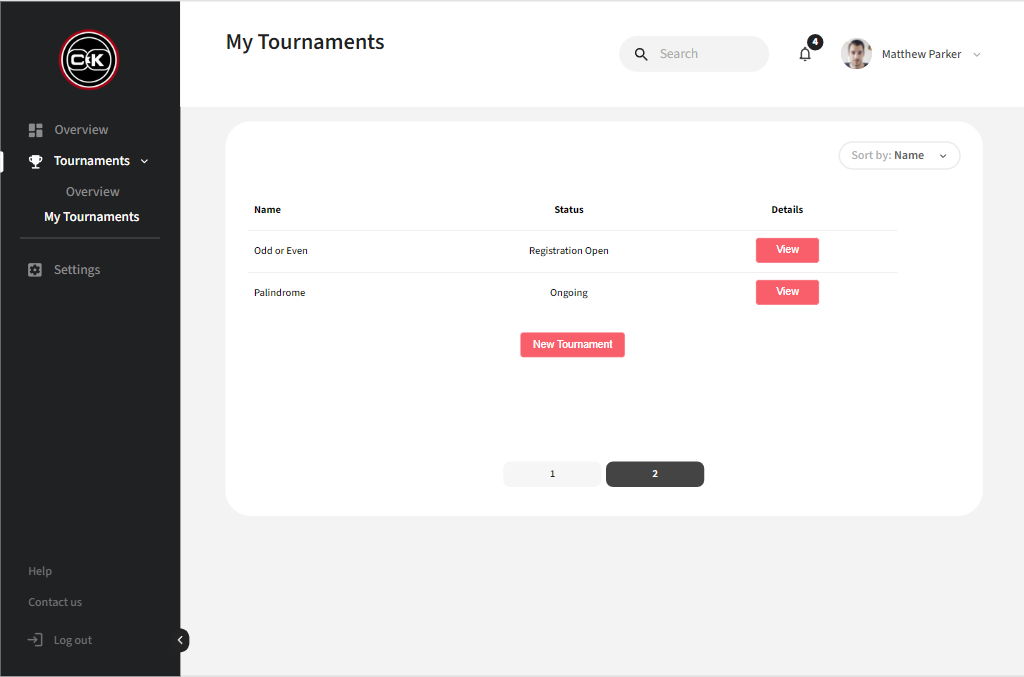
\includegraphics[width=\linewidth]{Web UI 3.png}
    \caption{Web UI My Tournament view}
\end{figure}

\begin{figure}[H]
    \centering
    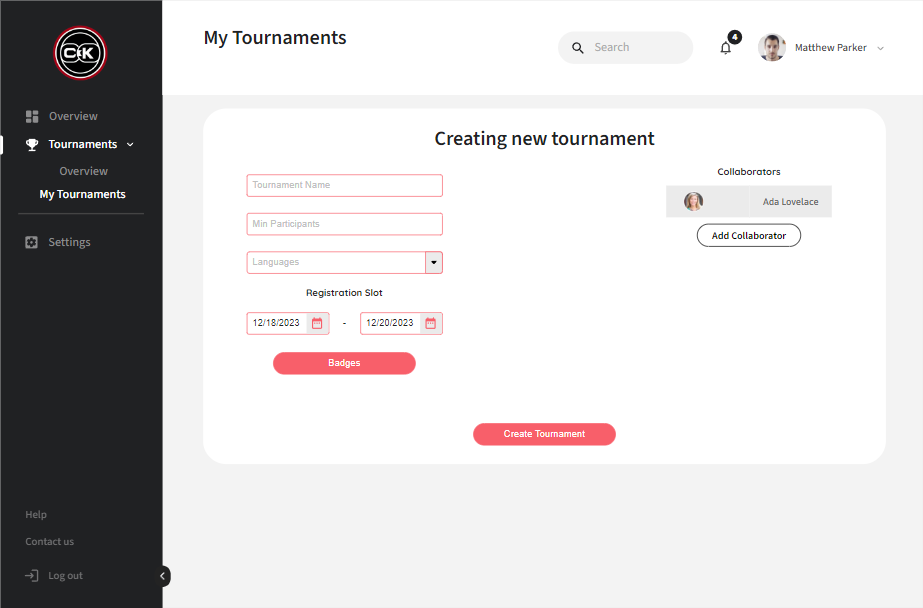
\includegraphics[width=\linewidth]{Web UI 4.png}
    \caption{Web UI Tournament creation view}
\end{figure}

\begin{figure}[H]
    \centering
    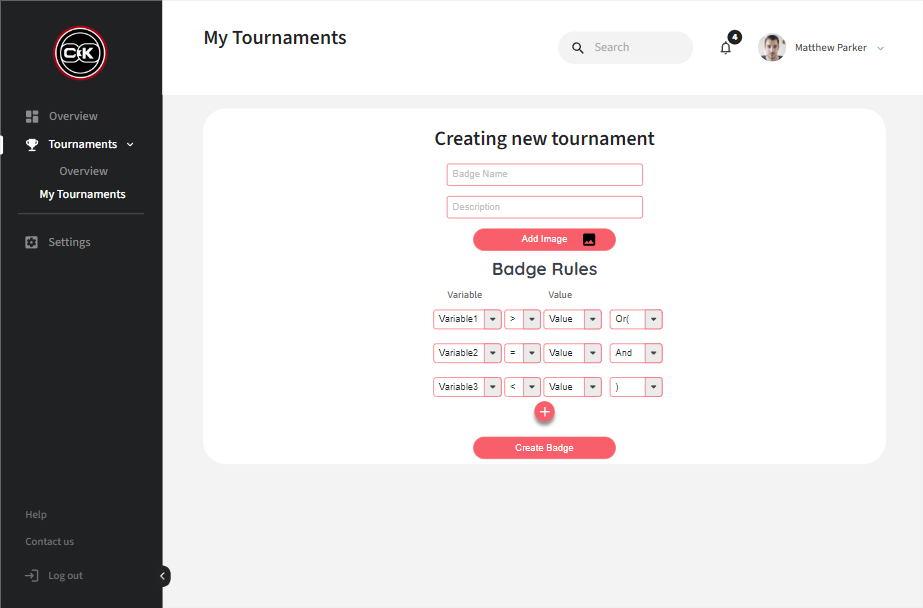
\includegraphics[width=\linewidth]{Web UI 5.png}
    \caption{Web UI Badge creation view}
\end{figure}
\newpage
\section{Requirements Traceability}
This section of the document details the design elements associated with each requirement outlined in the RASD. The following tables map these design elements to their respective requirements. \\

\begin{table}[H]
 \renewcommand{\arraystretch}{1.5}
    \centering
    \begin{tabular}{|l|p{10cm}|}
        \hline
        \textbf{Requirements} & $[FR1]$ The system allows Users to sign up \\
        \hline
        \textbf{Components} & 
        \begin{itemize}[align=left, topsep=0pt, partopsep=0pt]
            \item Smartphone App
            \item Web App
            \item Web Server
            \item Application Server:
            \begin{itemize}
                \item Dispatcher
                \item Registration Manager
                \item Model
            \end{itemize}
            \item Shared DBMS 
        \end{itemize} \\
        \hline
    \end{tabular}
\end{table}

\begin{table}[H]
 \renewcommand{\arraystretch}{1.5}
    \centering
    \begin{tabular}{|l|p{10cm}|}
        \hline
        \textbf{Requirements} & $[FR2]$ The system allows Users to log in \\
        \hline
        \textbf{Components} & 
        \begin{itemize}[align=left, topsep=0pt, partopsep=0pt]
            \item Smartphone App
            \item Web App
            \item Web Server
            \item Application Server:
            \begin{itemize}
                \item Dispatcher
                \item Login Manager
                \item Model
            \end{itemize}
            \item Shared DBMS 
        \end{itemize} \\
        \hline
    \end{tabular}
\end{table}

\begin{table}[H]
 \renewcommand{\arraystretch}{1.5}
    \centering
    \begin{tabular}{|l|p{10cm}|}
        \hline
        \textbf{Requirements} & $[FR3]$ The system allows Educators to create tournaments \\
        \hline
        \textbf{Components} & 
        \begin{itemize}[align=left, topsep=0pt, partopsep=0pt]
            \item Smartphone App
            \item Web App
            \item Web Server
            \item Application Server:
            \begin{itemize}
                \item Dispatcher
                \item Tournament Manager
                \begin{itemize}
                    \item Badge Manager
                    \item Battle Manager
                \end{itemize}
                \item Model
            \end{itemize}
            \item Shared DBMS 
        \end{itemize} \\
        \hline
    \end{tabular}
\end{table}

\begin{table}[H]
 \renewcommand{\arraystretch}{1.5}
    \centering
    \begin{tabular}{|l|p{10cm}|}
        \hline
        \textbf{Requirements} & 
        \vspace{-0.6cm}
        \begin{itemize}[label={}, left=0pt, align=left, itemsep=5pt]
            \item $[FR4]$ The system allows Educators to set a deadline for subscribing to the tournament
            \item $[FR5]$ The System allows Educators to set a list of programming languages that will be used in the tournament
            \item $[FR6]$ The system allows Educators to invite other Educators as collaborators for a tournament
            \item $[FR18]$ The system allows Students to join a tournament
            \item $[FR22]$ The system allows Educators to see the list of the active tournaments they have created
            \item $[FR23]$ The system allows Students to see the list of the active tournaments they have joined
        \end{itemize} \\
        \hline
        \textbf{Components} & 
        \begin{itemize}[align=left, topsep=0pt, partopsep=0pt]
            \item Smartphone App
            \item Web App
            \item Web Server
            \item Application Server:
            \begin{itemize}
                \item Dispatcher
                \item Tournament Manager
                \item Model
            \end{itemize}
            \item Shared DBMS 
        \end{itemize} \\
        \hline
    \end{tabular}
\end{table}

\begin{table}[H]
 \renewcommand{\arraystretch}{1.5}
    \centering
    \begin{tabular}{|l|p{10cm}|}
        \hline
        \textbf{Requirements} &
        \vspace{-0.6cm}
        \begin{itemize}[label={}, left=0pt, align=left, itemsep=5pt]
            \item $[FR7]$ The system allows Educators to set the number of battles in a tournament
            \item $[FR9]$ The system allows Educators to set a deadline for the subscription to the battle
            \item $[FR10]$ The system allows Educators to set a deadline for the submission of the solutions to the battle
            \item $[FR11]$ The System allows educators to choose which of the languages of the tournament will be used in each battle
            \item $[FR13]$ The system allows Educators to set the maximum number of students per team in a battle
            \item $[FR14]$ The system allows Educators to choose whether and when the scores will be assigned in a totally automatic way or also through a manual verification by themselves
            \item $[FR20]$ The system allows Students to join a battle
            \item $[FR21]$ The system allows Students to know about the provisional scores of all students, updated for every solution submitted, for all the duration of a battle
        \end{itemize} \\
        \hline
        \textbf{Components} & 
        \begin{itemize}[align=left, topsep=0pt, partopsep=0pt]
            \item Smartphone App
            \item Web App
            \item Web Server
            \item Application Server:
            \begin{itemize}
                \item Dispatcher
                \item Tournament Manager
                \begin{itemize}
                    \item Battle Manager
                \end{itemize}
                \item Model
            \end{itemize}
            \item Shared DBMS 
        \end{itemize} \\
        \hline
    \end{tabular}
\end{table}

\begin{table}[H]
 \renewcommand{\arraystretch}{1.5}
    \centering
    \begin{tabular}{|l|p{10cm}|}
        \hline
        \textbf{Requirements} &
        \vspace{-0.6cm}
        \begin{itemize}[label={}, left=0pt, align=left, itemsep=5pt]
            \item $[FR8]$ The system allows Educators to create battles
            \item $[FR12]$ The System allows Educators to upload the files with the text of the problem and test cases for the battle
        \end{itemize} \\
        \hline
        \textbf{Components} & 
        \begin{itemize}[align=left, topsep=0pt, partopsep=0pt]
            \item Smartphone App
            \item Web App
            \item Web Server
            \item Application Server:
            \begin{itemize}
                \item Dispatcher
                \item Tournament Manager
                \begin{itemize}
                    \item Battle Manager
                \end{itemize}
                \item Model
            \end{itemize}
            \item GitHub
            \item Shared DBMS 
        \end{itemize} \\
        \hline
    \end{tabular}
\end{table}

\begin{table}[H]
 \renewcommand{\arraystretch}{1.5}
    \centering
    \begin{tabular}{|l|p{10cm}|}
        \hline
        \textbf{Requirements} &
        \vspace{-0.6cm}
        \begin{itemize}[label={}, left=0pt, align=left, itemsep=5pt]
            \item $[FR15]$ The system allows Educators to create badges for a specific tournament
            \item $[FR16]$ The system allows Educators to build the requirements for achieving a badge
            \item $[FR17]$ The system allows Students to see what are the active badges in a tournament and what they have to do to achieve them
        \end{itemize} \\
        \hline
        \textbf{Components} & 
        \begin{itemize}[align=left, topsep=0pt, partopsep=0pt]
            \item Smartphone App
            \item Web App
            \item Web Server
            \item Application Server:
            \begin{itemize}
                \item Dispatcher
                \item Tournament Manager
                \begin{itemize}
                    \item Badge Manager
                \end{itemize}
                \item Model
            \end{itemize}
            \item Shared DBMS 
        \end{itemize} \\
        \hline
    \end{tabular}
\end{table}

\begin{table}[H]
 \renewcommand{\arraystretch}{1.5}
    \centering
    \begin{tabular}{|l|p{10cm}|}
        \hline
        \textbf{Requirements} & $[FR19]$ The system allows Students to invite other students to form teams for a battle \\
        \hline
        \textbf{Components} & 
        \begin{itemize}[align=left, topsep=0pt, partopsep=0pt]
            \item Smartphone App
            \item Web App
            \item Web Server
            \item Application Server:
            \begin{itemize}
                \item Dispatcher
                \item Tournament Manager
                \begin{itemize}
                    \item Battle Manager
                \end{itemize}
                \item Model
                \item Notification Manager
            \end{itemize}
            \item Shared DBMS 
        \end{itemize} \\
        \hline
    \end{tabular}
\end{table}

\begin{table}[H]
 \renewcommand{\arraystretch}{1.5}
    \centering
    \begin{tabular}{|l|p{10cm}|}
        \hline
        \textbf{Requirements} &
        \vspace{-0.6cm}
        \begin{itemize}[label={}, left=0pt, align=left, itemsep=5pt]
            \item $[FR24]$ The system allows Users to see the stats of any other account registered in the system
            \item $[FR25]$ The system allows Users to search for other accounts or tournaments on the search bar
        \end{itemize} \\
        \hline
        \textbf{Components} & 
        \begin{itemize}[align=left, topsep=0pt, partopsep=0pt]
            \item Smartphone App
            \item Web App
            \item Web Server
            \item Application Server:
            \begin{itemize}
                \item Dispatcher
                \item Search Manager
                \item Model
            \end{itemize}
            \item Shared DBMS 
        \end{itemize} \\
        \hline
    \end{tabular}
\end{table}

\section{Implementation, Integration and Test Plan}
\subsection{Overview}
\subsection{Implementation Plan}
\subsubsection{Features Identification}
The system's features are directly derived from the system requirements. It's worth noting that some features necessitate the implementation of entire components, while others involve smaller portions. Below is a brief recap of the system's features. \\\\
\textbf{[F1] Sign in and Sign up} \\
These features allow users to access the system, it is important to notice that the implementation is the same for both students and educators since they will access the system in the same way. \\\\
\textbf{[F2] Badge Management} \\
This feature serves as a core component of the Tournament Manager, managed by the Badge Manager. Although badges are not mandatory for creating a tournament, this component plays a crucial role in the tournament creation process. \\\\
\textbf{[F3] Battle Management} \\
This feature is a core component of the Tournament Manager, managed by the Battle Manager. It plays a crucial role in the creation of a tournament since tournaments without battles cannot exist. Therefore, this component is mandatory for the creation of a tournament. \\\\
\textbf{[F4] Tournament Management} \\
This feature stands as the central component of the system, provided by the Tournament Manager and its sub-components, namely the Badge Manager and Battle Manager. Seamless operation of the Tournament Manager necessitates the integration of GitHub and CodeScene via API. \\\\
\textbf{[F5] User Notification} \\
The Notification Manager provides this feature, allowing the system to send notifications to users on both the Web App and Smartphone App. Additionally, invitations to join tournaments or battles are shared as notifications through the Notification Manager. \\\\
\textbf{[F6] Searching} \\
This feature is provided by the Search Manager and allows users to search for other users or tournaments.

\subsection{Components Integration and Testing}

\section{Effort Spent}
\begin{center}
\textbf{Armando Fiorini} \\
\vspace{10px}
    \begin{tabularx}{0.8\textwidth} { 
  | >{\centering\arraybackslash}X 
  | >{\centering\arraybackslash}X | }
 \hline
 \textbf{Chapter} & \textbf{Hours Spent} \\
 \hline
 1 & TBD  \\
 \hline
 2 & TBD \\
 \hline
 3 & TBD \\
 \hline
 4 & TBD \\
 \hline
 5 & TBD \\
 \hline
\end{tabularx}

\vspace{10px}
\textbf{Samuele Motta} \\
\vspace{10px}
\begin{tabularx}{0.8\textwidth} { 
  | >{\centering\arraybackslash}X 
  | >{\centering\arraybackslash}X | }
 \hline
 \textbf{Chapter} & \textbf{Hours Spent} \\
 \hline
 1 & TBD  \\
 \hline
 2 & TBD \\
 \hline
 3 & TBD \\
 \hline
 4 & TBD \\
 \hline
 5 & TBD \\
 \hline
\end{tabularx}

\vspace{10px}
\textbf{Vajihe Gholami} \\
\vspace{10px}
\begin{tabularx}{0.8\textwidth} { 
  | >{\centering\arraybackslash}X 
  | >{\centering\arraybackslash}X | }
 \hline
 \textbf{Chapter} & \textbf{Hours Spent} \\
 \hline
 1 & TBD  \\
 \hline
 2 & TBD \\
 \hline
 3 & TBD \\
 \hline
 4 & TBD \\
 \hline
 5 & TBD \\
 \hline
\end{tabularx}

\end{center}

\section{References}
\begin{itemize}
    \item Diagrams made with: StarUML and draw.io
    \item Mockups made with: moqups.com
\end{itemize}
\end{document}
